\documentclass[11pt]{amsart}

\usepackage{amsmath,amssymb,graphicx,bbm}
\usepackage{amsthm,verbatim}
\usepackage{mathrsfs,mathtools}
\usepackage{enumerate}
\usepackage{listings}
\usepackage{tikz}
\usetikzlibrary{arrows,automata}
\usepackage[footnotesize,bf]{caption}
\usepackage[left=1.1in,right=1.1in,top=1in]{geometry}

%\usepackage{mathdefs}

%% Patch for amsart date
\usepackage{etoolbox}
\makeatletter
\patchcmd{\@maketitle}
  {\ifx\@empty\@dedicatory}
  {\ifx\@empty\@date \else {\vskip3ex \centering\footnotesize\@date\par\vskip1ex}\fi
   \ifx\@empty\@dedicatory}
  {}{}
\patchcmd{\@adminfootnotes}
  {\ifx\@empty\@date\else \@footnotetext{\@setdate}\fi}
  {}{}{}
\makeatother

\title{HW 3: Data Dependences}
\author{Dihan Dai}
\date{\today}

\begin{document}
\maketitle
\section*{Question 1}
\begin{enumerate}[(a)]
\item The validity condition for loop unrolling is that the dependence vector of permutation corresponding to moving the unrolled loop to the innermost loop is valid. Therefore, 
\begin{itemize}
\item $(0, 0, 1, -1)$: unrolling t, i and k loops is valid.
\item $(1, -2, 1, -1)$: unrolling i, j and k loops is valid.
\item $(1, -1, 1, 0)$: unrolling i, j and k loops is valid.
\end{itemize}
\item The validity condition for loop permutation is that the dependence vector of the corresponding permutation is valid.
\begin{itemize}
\item $(0, 0, 1, -1)$: tijk, itjk, tjki, ijkt, jkti, jkit, tjik, ijtk, jtki, jikt, jitk, jtik
\item $(1, -2, 1, -1)$: tijk, tikj, tjki, tjik, tkij, tkji, jtik, jtki, jkit, jkti, jitk, jikt
\item $(1, -1, 1, 0)$:  tijk, tikj, tjki, tjik, tkij, tkji, jtik, jtki, jkit, jkti, jitk, jikt, ktji, ktij, kjti, kjit
\end{itemize}
\item The vaidity condition for loop tiling is that the corresponding loops are fully permutable.
\begin{itemize}
\item $(0, 0, 1, -1)$: 3D tiling: tij, 2D tiling: ti, tj, ij,
\item $(1, -2, 1, -1)$: 3D tiling: ijk, 2D tiling: tj, ij, ik, jk,
\item $(1, -1, 1, 0)$:  3D tiling: ijk, 2D tiling: tj, ij, ik, jk,
\end{itemize}
\end{enumerate}
\newpage
\section*{Question 2}
\begin{enumerate}[(a)]
\item Yes. If there is an output dependences between $(t_1,i_1,j_1)$ and $(t_2,i_2,j_2)$ such that $(t_1,i_1,j_1)<(t_2,i_2,j_2)$, it must satisfy $(i_1+1, j_1-1) = (i_2+1, j_2-1)$. The dependence vectors are given by $(t_2-t_1,i_2-i_1,j_2-j_1)$ and the smallest of such vectors is $(1, 0, 0)$. The leftmost nonzero element of the vector is positive, thus the dependence vector is valid.
\item 
\begin{itemize}
\item Flow dependence: if there is a flow dependeces between the write instance $(t_w, i_w, j_w)$ and the read instance$(t_r, i_r, j_r)$. The dependences vector are given by $(t_r-t_w,i_r-i_w,j_r-j_w)$ and they must satisfies
\begin{itemize}
\item either $(i_r,j_r+1) = (i_w+1,j_w-1)$, where the smallest dependence vector is $(0,1,-2)$,
\item or $(i_r-1,j_r) = (i_w+1,j_w-1)$, where the smallest dependence vector is $(0,2,-1)$.
\end{itemize}
Both dependence vectors are valid because the leftmost nonzero elements of both vectors are positive.
\item Anti-dependence: if there is an anti-dependeces between the read instance$(t_r, i_r, j_r)$ and the write instance $(t_w, i_w, j_w)$. The dependences vector are given by $(t_w-t_r,i_w-i_r,j_w-j_r)$ and they must satisfies
\begin{itemize}
\item either $(i_r,j_r+1) = (i_w+1,j_w-1)$, where the smallest dependence vector is $(1,-1,2)$,
\item or $(i_r-1,j_r) = (i_w+1,j_w-1)$, where the smallest dependence vector is $(1,-2,-1)$.
\end{itemize}
Both dependence vectors are valid because the leftmost nonzero elements of both vectors are positive.
\end{itemize}
\end{enumerate}
\newpage
\section*{Question 3}
\begin{enumerate}[(i)]
\item 
\begin{align*}
\text{i loop: } S1[i,j,k]\to S3[i+1,j,k], \\
\text{k loop: } S2[i,j,k]\to S1[i,j,k+1], \\
\text{j loop: }S3[i,j,k]\to S2[i,j+1,k].
\end{align*}
\item No parallelization can be achieved since every loop carries dependence.
\item No. It is because the dependences of every loop doesn't change no matter what permutation of the nested loops is.
\end{enumerate}
\vfill
\section*{Question 4}
\begin{enumerate}[(i)]
  \item Dependence graph:

  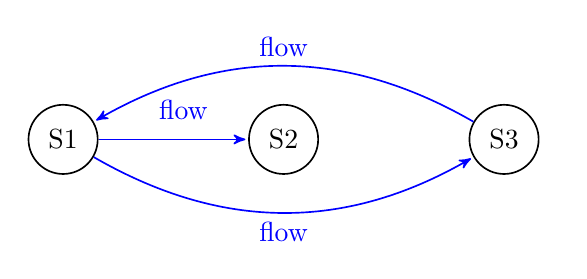
\begin{tikzpicture}[->,>=stealth',shorten >=1pt,auto,node
    distance=2.8cm, semithick]
  
    \node[state, label=below:{}] (A) {S1};
    \node[state, label=left:{}] (B) [right of=A] {S2};
    \node[state, label=right:{}] (C) [right of=B] {S3};
  
    \path 
    (A) edge [blue] node[right, label=above:{flow}] {} (B)
    (A) edge [bend right, blue] node[label=below:{flow}] {} (C)
    (C) edge [bend right, blue] node[label=above:{flow}] {} (A);
  \end{tikzpicture}
    \begin{align*}
      &S1[i]\xrightarrow[]{\text{flow}} S2[i]\\
      &S1[i]\xrightarrow[]{\text{flow}} S3[i+1]\\
      &S3[i]\xrightarrow[]{\text{flow}} S1[i+1]
    \end{align*}
    Statement 1 and 3 form a cycle, thus only statement 2 can be vectorized.
  \item 
  \begin{lstlisting}[language = c]
        for(i=1; i<256; i++)
        {
            a[i] = c[i]+1;
            c[i+1] = a[i-1]+1;
        }

        b[1:255] = a[1:255]-1;
  \end{lstlisting}
\end{enumerate}
\vfill
\section*{Question 5}
\begin{enumerate}[(i)]
\item Data dependences:
\begin{align*}
& S[i,j,k]\to S[i+1,j-1,k-1] \text{ flow}\\
\end{align*}
\item
\begin{lstlisting}[language = c]
  for(i=1; i<256; i++)
  {
    a[i][1:255][1:255] = a[i-1][2:256][2:256]+1;
  }
\end{lstlisting}
\end{enumerate}
\vfill
\end{document}
